\begin{homeworkProblem}
  \begin{enumerate}[a)]
    \item Simplifique el algoritmo de eliminación de Gauss de manera adecuada para resolver un sistema lineal $Ax=b$ con
    \[
      A = \begin{pmatrix}
        a_{11} & a_{12} &  &  &  \\
        a_{12} & a_{22} & a_{23} &  &  \\
        & a_{23} & \ddots & \ddots &  \\
        &  & \ddots & a_{n-1,n-1} & a_{n-1,n} \\
        &  &  & a_{n-1,n} & a_{n,n}
      \end{pmatrix}\in \mathbb{R}^{n \times n}
    \]
    matriz tridiagonal.
    \item Considere la ecuación de Poisson con término fuente $f$ en el intervalo $(0,1)$:
    \begin{align*}
      -T"(x)=f(x), x \in (0,1),
    \end{align*}
    con condiciones de frontera $T(0)=T(1)=0$. Para resolver numéricamente el problema de valor en la frontera, la segunda derivada de T se aproxima por medio de diferencias finitas con un paso de discretización $h>0$:
    \begin{align*}
      T"(x)\approx \frac{T(x-h)-2T(x)+T(x+h)}{h^2}
    \end{align*}
    Tomando $x_i=ih$, $i=0, 1, \dotsc, n$, $n=1/h$, obtenemos el sistema lineal de ecuaciones
    \begin{align*}
      -T_{i-1}+2T_i-T_{i+1}=h^2f(x_i), \hspace{1cm} i=1, \dotsc, n-1   \hspace{3cm} \text{(1)}
    \end{align*}
    para las incognitas $T_i\approx T(x_i)$, $i=1, \dotsc, n-1$ (de las condiciones de frontera se tiene que $T_0=T_n=0$).
    Escriba $(1)$ en la forma $AT=f$ donde $A$ es una matriz tridiagonal. Utilice su algoritmo desarrollado en la parte $a)$ para resolver el sistema lineal de ecuaciones para $n=1000$ y $f(x)=\text{sen}(2\pi x)/(4\pi^2)$.
  \end{enumerate}
  \begin{solucion}
    \begin{enumerate}[a)]
      \item Con el objetivo de simplificar el algoritmo de eliminación de Gauss, tomemos como base el algoritmo presentado en clase y la representación general de la matriz A,\\
        \textbf{Algoritmo de eliminación de Gauss:}\\
        \noindent
        \begin{minipage}[t]{0.6\textwidth}
          Para $k = 1, 2, \dotsc, n-1$: \\
          \phantom{Para} Para $i = k+1, k+2, \dotsc, n$: \\
          \phantom{Para Para} $m_{ik} = \frac{a_{ik}^{(k)}}{a_{kk}^{(k)}}$ \\
          \phantom{Para Para} Para $j = k+1, k+2, \dotsc, n$: \\
          \phantom{Para Para Para} $a_{ij}^{(k+1)} = a_{ij}^{(k)} - m_{ik}a_{kj}^{(k)}$ \\
          \phantom{Para Para Para} $b_{i}^{(k+1)} = b_{i}^{(k)} - m_{ik}b_{k}^{(k)}$ \\
          Para $i = n, n-1, \dotsc, 1$: \\
          \phantom{Para} $x_i = \frac{1}{a_{ii}^{(i)}}\left( b_i^{(i)} - \sum_{j=i+1}^n a_{ij}^{(i)}x_j\right)$
        \end{minipage}%
        \hspace{-1cm}% Espacio entre columnas ajustado
        \begin{minipage}[t]{0.35\textwidth}
          \[
            A = \begin{pmatrix}
              \ddots & \ddots &  &  &  \\
              \ddots & a_{kk} & a_{k,k+1} &  &  \\
              & 0 & a_{k+1,k+1}^{(k)} & a_{k+1,k+2}^{(k)} &  \\
              &  & a_{k+2,k+1}^{(k)} & a_{k+2,k+2}^{(k)} & \ddots \\
              &  &  & \ddots & \ddots
            \end{pmatrix}
          \]
        \end{minipage}\\
        En primera instancia, eliminaremos el segundo contador ($i = k+1, k+2, \dotsc, n$), pues la única componente $a_{ik}^{(k)}$ presuntamente distinta de cero es $i = k+1$. Por ende, el contador es innecesario. \\
        Además, eliminaremos también el tercer contador ($j = k+1, k+2, \dotsc, n$), ya que dichas operaciones realizan la eliminación entre filas, necesaria únicamente para las componentes de la fila $k$-ésima presuntamente distintas de cero, lo cual solo ocurre para $a_{k,k+1}^{(k)}$. Por lo tanto, el contador es descartado. Es importante recalcar que $a_{k+1,k+2}^{(k+1)} = a_{k+1,k+2}^{(k)}$. \\
        Finalmente, conservaremos el último contador, pero modificaremos la sumatoria. Esto se debe a que, después de realizar la eliminación de Gauss, por cada fila solo habrá dos componentes distintas de cero: $a_{ii}^{(i)}$ y $a_{i,i+1}^{(i)}$. En consecuencia, la sumatoria no es necesaria.\\
        Por consiguiente, el \textbf{Algoritmo de eliminación de Gauss modificado} queda de la siguiente forma:\\
          Para $k = 1, 2, \dotsc, n-1$: \\
          \phantom{Para} $m_{k+1,k} = \frac{a_{k+1,k}^{(k)}}{a_{kk}^{(k)}}$ \\
          \phantom{Para} $a_{k+1,k+1}^{(k+1)} = a_{k+1,k+1}^{(k)} - m_{k+1,k}a_{k,k+1}^{(k)}$ \\
          \phantom{Para} $a_{k+1,k+2}^{(k+1)} = a_{k+1,k+2}^{(k)}$ \\
          \phantom{Para} $b_{k+1}^{(k+1)} = b_{k+1}^{(k)} - m_{k+1,k}b_{k}^{(k)}$ \\
          Para $i = n-1, \dotsc, 1$: \\
          \phantom{Para} $x_n = \frac{b_n^{(n)}}{a_{nn}^{(n)}}$ \\
          \phantom{Para} $x_i = \frac{1}{a_{ii}^{(i)}}\left( b_i^{(i)} - a_{i,i+1}^{(i)}x_{i+1}\right)$
        \item Siguiendo las intrucciones enunciadas obtenemos el sistema lineal de ecuaciones.\\ 
          \[
            \begin{cases}
              -T_{0} + 2T_1 -T_2= h^2 f(x_1), \\
              -T_{1} + 2T_2 -T_3= h^2 f(x_2), \\
              \hspace{1cm} \vdots \hspace{3cm} \vdots \\
              -T_{n-2} + 2T_{n-1} -T_n= h^2 f(x_{n-1}).
            \end{cases}
          \]
          donde $x_i=ih$, $i=0, 1, \dotsc, n$, $n=1/h$ y  $T_i\approx T(x_i)$, $i=1, \dotsc, n-1$ (con condiciones de frontera $T_0=T_n=0$). Luego con dichas condiciones el sistema lineal queda de la siguiente forma:
          \[
            \begin{cases}
              2T_1 -T_2= h^2 f(x_1), \\
              -T_{1} + 2T_2 -T_3= h^2 f(x_2), \\
              \hspace{1cm} \vdots \hspace{3cm} \vdots \\
              -T_{n-2} + 2T_{n-1} = h^2 f(x_{n-1}).
            \end{cases}
          \]
          Por ende en forma matricial, $AT=f$,
          \[
            \begin{pmatrix}
              2 & -1 & 0 & \dots & 0 \\
              -1 & 2 & -1 & \dots & 0 \\
              0 & -1 & 2 & \dots & 0 \\
              \vdots & \vdots & \vdots & \ddots & \vdots \\
              0 & 0 & \dots & 2 & -1\\
              0 & 0 & \dots & -1 & 2
              \end{pmatrix}
              \begin{pmatrix}
              T_1 \\
              T_2 \\
              T_3 \\
              \vdots \\
              T_{n-1}
              \end{pmatrix}
              =
              \begin{pmatrix}
              h^2 f(x_1) \\
              h^2 f(x_2) \\
              h^2 f(x_3) \\
              \vdots \\
              h^2 f(x_{n-1})
            \end{pmatrix}.
          \]
          Ahora en nuestro caso particular tomando $n=1000$ y $f(x)=\text{sen}(2\pi x)/(4\pi^2)$, el algoritmo queda de la siguiente forma:
          \begin{lstlisting}
import numpy as np
            
n = 1000 # Tamano de la matriz
c = -1  # Numero que deseas en la diagonal superior e inferior inmediata
a = 2  # Numero que deseas en la diagonal principal
            
            
# Crear matriz de ceros
matriz = np.zeros((n, n))
            
# Llenar la diagonal superior e inferior inmediata
for i in range(n - 1):
  matriz[i, i + 1] = c
  matriz[i + 1, i] = c
            
# Llenar la diagonal principal
for i in range(n):
  matriz[i, i] = a
            
print(matriz)
          \end{lstlisting}
          \begin{center}[h]
            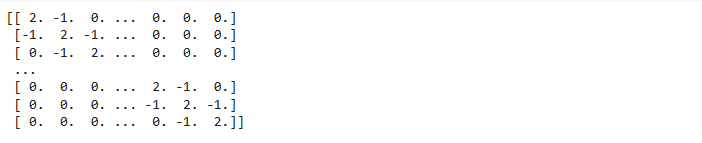
\includegraphics[scale=0.5]{code1.png}
          \end{center}
          \begin{lstlisting}
# Definimos f(x)
def funcion(x):
  return np.sin(2 * np.pi * x)
            
# Definimos h para la matriz
h=1/n
            
# definimos nuestro vactor independiente
valores = []  # Lista con valores especificos
for i in range(1, n + 1):
  valores.append((h ** 2) * funcion(i * h))
            
# Convertir la lista en un vector columna nx1
b = np.array(valores).reshape(n, 1)  # Convertirlos en vector columna nx1
print(b[:5])
          \end{lstlisting}
          \begin{center}
            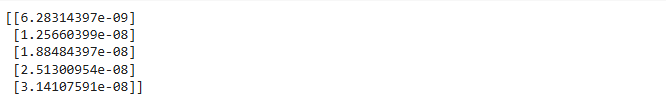
\includegraphics[scale=1]{code2.png}
          \end{center}
          \begin{lstlisting}
# Eliminacion de Gauss simplificado para tridiagonales
for i in range(n-1):
  multiplicador = matriz[i + 1, i] / matriz[i, i]                      # Encontrando los multiplicadores para la fila i+1
  matriz[i + 1 ,i] = 0
  matriz[i + 1, i + 1] = matriz[i + 1, i + 1] - multiplicador * matriz[i, i + 1]  # Actualizando la fila i+1
  b[i + 1] = b[i + 1] - multiplicador * b[i]   # Aplicando la operacion al termino independiente
  print("Matriz despues de aplicarle eliminacion de Gauss (primeros 5 filas):")
print(matriz)
          \end{lstlisting}
          \begin{center}
            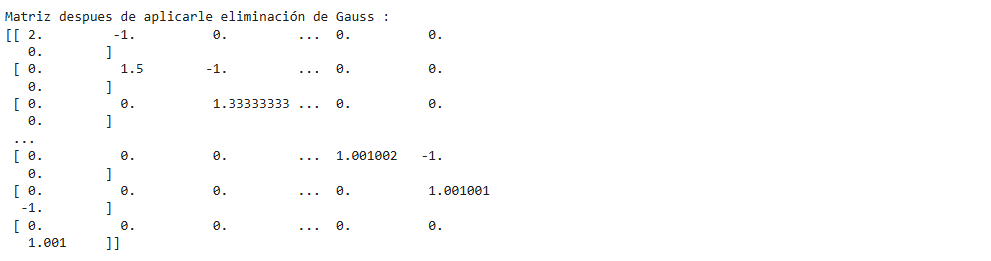
\includegraphics[scale=1]{code3.png}
          \end{center}
          \begin{lstlisting}
print("Termino independiente b (primeros 5 valores):")
print(b[:5])
          \end{lstlisting}
          \begin{center}
            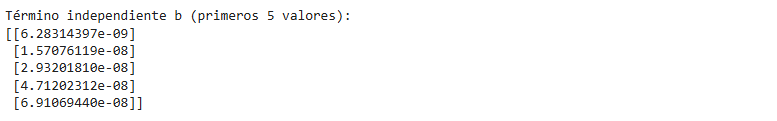
\includegraphics[scale=1]{code4.png}
          \end{center}
          \begin{lstlisting}
# Sustitución regresiva simplificada
x = np.zeros((n, 1))  # Crear el vector solucion
            
for j in range(n - 1, -1, -1):  # Desde la ultima fila hasta la primera
  if j == n - 1:              # Caso base: ultima fila
    x[j] = b[j] / matriz[j, j]
  else:
    x[j] = (b[j] - matriz[j, j + 1] * x[j + 1]) / matriz[j, j]
            
print("Solucion x (primeros 5 valores):")
print(x[:5])            
          \end{lstlisting}
          \begin{center}
            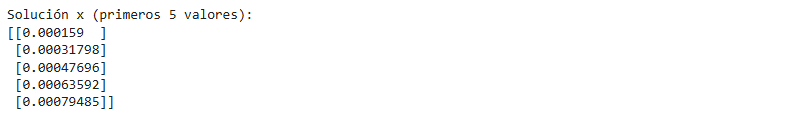
\includegraphics[scale=0.7]{code5.png}
          \end{center}
          \begin{lstlisting}
# Definimos la funci0n real
def funcion_real(x):
  return np.sin(2 * np.pi * x) / (4 * (np.pi ** 2))
            
# Definimos la funcion Error Absoluto
  def error_absoluto(x, h):
    # Creamos una copia para no modificar la original
    errores = np.zeros_like(x)  # Vector de errores
    valores_T1 = np.zeros_like(x)  # Vector para almacenar los valores de T_1
            
    for i in range(len(x)):
      T_1 = funcion_real((i + 1) * h)  # Calcula el valor real
      valores_T1[i] = T_1  # Guarda el valor de T_1 en el vector
      errores[i] = abs(T_1 - x[i])  # Calcula el error absoluto
            
    return errores, valores_T1, x
  values = np.zeros((n,1))
  for i in range(1000):
    values[i] = (i+1) * h

  # Llamamos a la funcion
  errores, valores_T1, x = error_absoluto(x, h)
            
  # Mostramos los resultados
  print("Valores reales T_1 (primeros 5 valores):")
  print(valores_T1[:5])
  print("\nError absoluto (primeros 5 valores):")
  print(errores[:5])        
          \end{lstlisting}      
          \begin{center}
            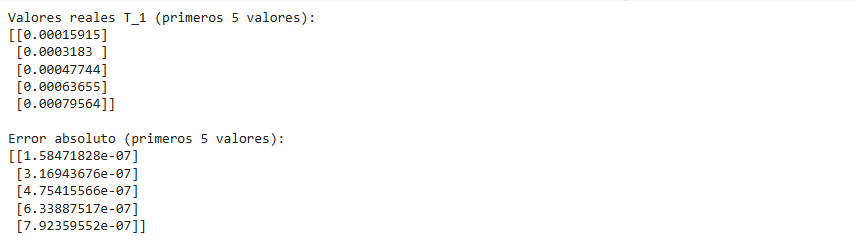
\includegraphics[scale=0.8]{code6.png}
          \end{center}
          \begin{lstlisting}
import pandas as pd
import matplotlib.pyplot as plt

tabla = pd.DataFrame({
    "x": values.flatten(),
    "T_1": valores_T1.flatten(),
})
# Supongamos que `tabla` ya está creada con tus datos
plt.figure(figsize=(10, 6))

# Graficar T_1
plt.plot(tabla['x'], tabla['T_1'], label='T_1', marker='o', linestyle='-', color='b')

# Personalizar la gráfica
plt.title('Gráfica de T_1')
plt.xlabel('x')
plt.ylabel('T_1')
plt.grid(True)
plt.legend()
plt.show()
print(tabla.head(1000))
          \end{lstlisting}
          \begin{center}
            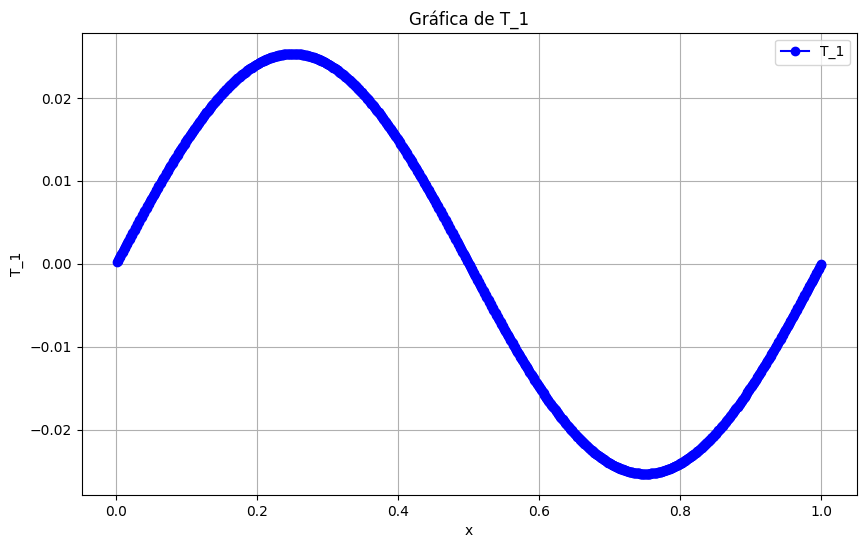
\includegraphics[scale=0.6]{grafica_T1.png}\\
            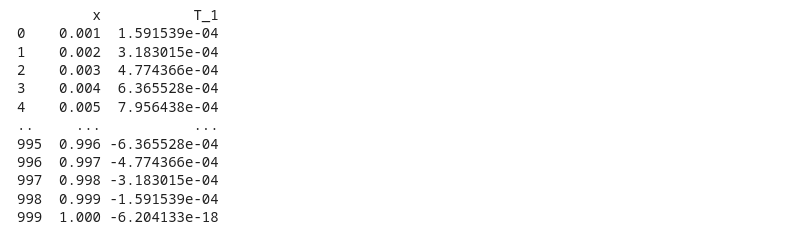
\includegraphics[scale=1]{code7.png}
          \end{center}
          \newpage
          \begin{lstlisting}
tabla = pd.DataFrame({
    "x": values.flatten(),
    "approx": x.flatten(),
})
# Supongamos que `tabla` ya está creada con tus datos
plt.figure(figsize=(10, 6))

# Graficar x
plt.plot(tabla['x'], tabla['approx'], label='approx', marker='o', linestyle='-', color='b')

# Personalizar la gráfica
plt.title('Gráfica de la aproximacion')
plt.xlabel('x')
plt.ylabel('approx')
plt.grid(True)
plt.legend()
plt.show()
print(tabla.head(1000))  
          \end{lstlisting}
          \begin{center}
            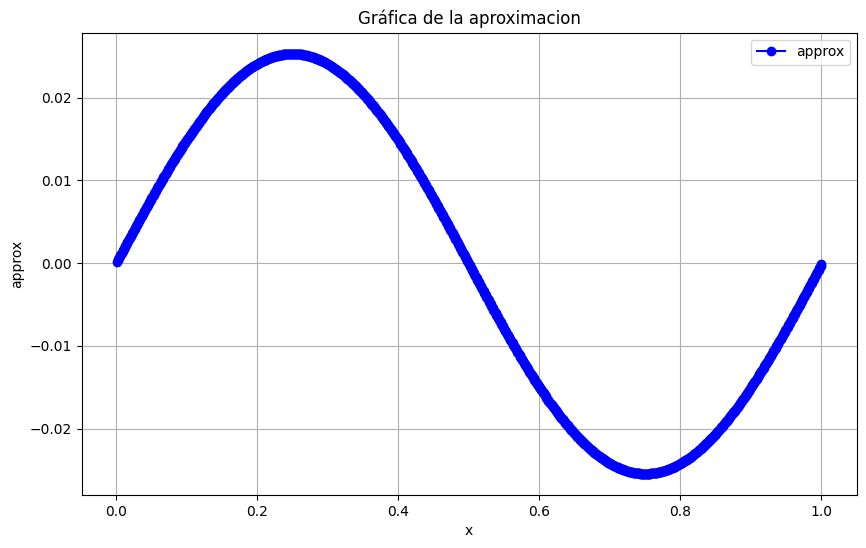
\includegraphics[scale=0.6]{grafica_approx.png}\\
            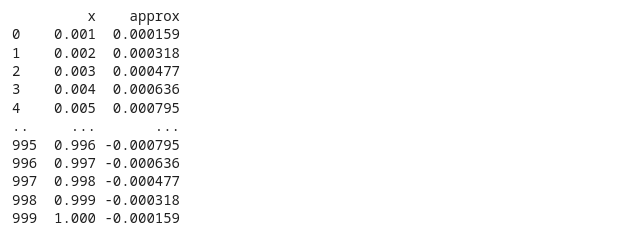
\includegraphics[scale=1]{code8.png}
          \end{center}
          \begin{lstlisting}
tabla = pd.DataFrame({
    "x": x.flatten(),
    "T_1": valores_T1.flatten(),
    "Error Absoluto": errores.flatten()
})
print(tabla.head(1000))  
          \end{lstlisting}
          \begin{center}
            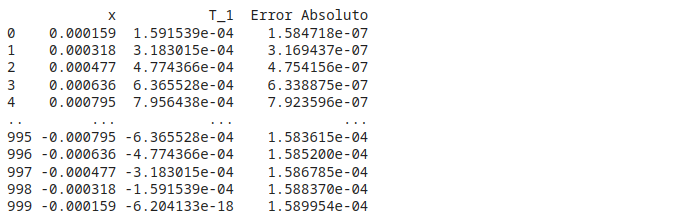
\includegraphics[scale=1]{code9.png}  
          \end{center}
          \newpage
          Usando Python para cálcular el número de condición se tiene que:
          \begin{lstlisting}
condicion = np.linalg.cond(matriz)
print("Número de condición:", condicion)  
          \end{lstlisting}
          en dónde la salida es:\\
          Número de condición: $782.9164494157501$.\\
          Cuando se utiliza \( n = 1000 \), la propagación de errores debido a la eliminación modificada y la sustitución hacia atrás de Gauss es extremadamente alta, lo que provoca que la aproximación tenga un error cercano al 99\%. Esto se debe a que, al ser tan grande el valor de \( n \), el tamaño de paso \( h \) es muy pequeño, lo que introduce errores de truncamiento en cada operación del proceso de solución. Estos errores se acumulan a lo largo de las iteraciones, amplificando la inexactitud de la solución final. 
          El comportamiento observado sugiere que, aunque el método parece adecuado para valores más pequeños de \( n \), al aumentar el número de nodos, el método no es suficientemente preciso debido a la acumulación de errores en las operaciones, lo que limita su eficacia a medida que la discretización se afina. Esto destaca la importancia de encontrar un balance adecuado entre la resolución del problema y la precisión numérica para evitar la propagación excesiva de errores.
    \end{enumerate}
  \end{solucion}
\end{homeworkProblem}
